\documentclass[varwidth,border=10pt]{standalone}

\usepackage[aboveskip=1pt,labelfont=bf,labelsep=period,justification=raggedright,singlelinecheck=off]{caption}
\usepackage{amsmath}
\usepackage{tikz}
\usepackage{tikz-cd}
\usetikzlibrary{matrix,arrows,positioning,calc,shapes,arrows.meta}
\usepackage{xstring}
\tikzset{  
	-Latex,auto,node distance =1.5 cm and 1.3 cm, thick,% node distance is the distance between one node to other, where 1.5cm is the length of the edge between the nodes  
	state/.style ={ellipse, draw, minimum width = 0.9 cm}, % the minimum width is the width of the ellipse, which is the size of the shape of vertex in the node graph  
	point/.style = {circle, draw, inner sep=0.18cm, fill, node contents={}},  
	bidirected/.style={Latex-Latex,dashed}, % it is the edge having two directions  
	el/.style = {inner sep=2.5pt, align=right, sloped}  
} 
%\usepackage[subrefformat=parens, labelfont=up]{subcaption}
%\usepackage{cleveref}
%\crefname{thm}{Theorem}{Theorems}
\setlength{\textwidth}{\dimexpr 6in\relax}
\usepackage{makecell}



\newcommand{\bbB}{\mathbb{B}}
\newcommand{\bL}{\mathbb{L}}
\newcommand{\bU}{\mathbb{U}}

\newcommand{\cL}{\mathcal{L}}
\newcommand{\cM}{\mathcal{M}}

\newcommand{\Targets}{\mathbf{T}}
\newcommand{\Sources}{\mathbf{S}}

\newcounter{countitems}


\newcommand{\boolf}{{\mathfrak 0}}
\newcommand{\boolt}{{\mathfrak 1}}

\newcommand{\bzero}{{\bf 0}}
\newcommand{\bone}{{\bf 1}}

\newcommand{\setof}[1]{\left\{ {#1}\right\}}
\newcommand{\setdef}[2]{\left\{{#1}\,\left|\,{#2}\right.\right\}}

\usepackage[subrefformat=parens, labelfont=up]{subcaption}

\begin{document}

\begin{figure}
\centering
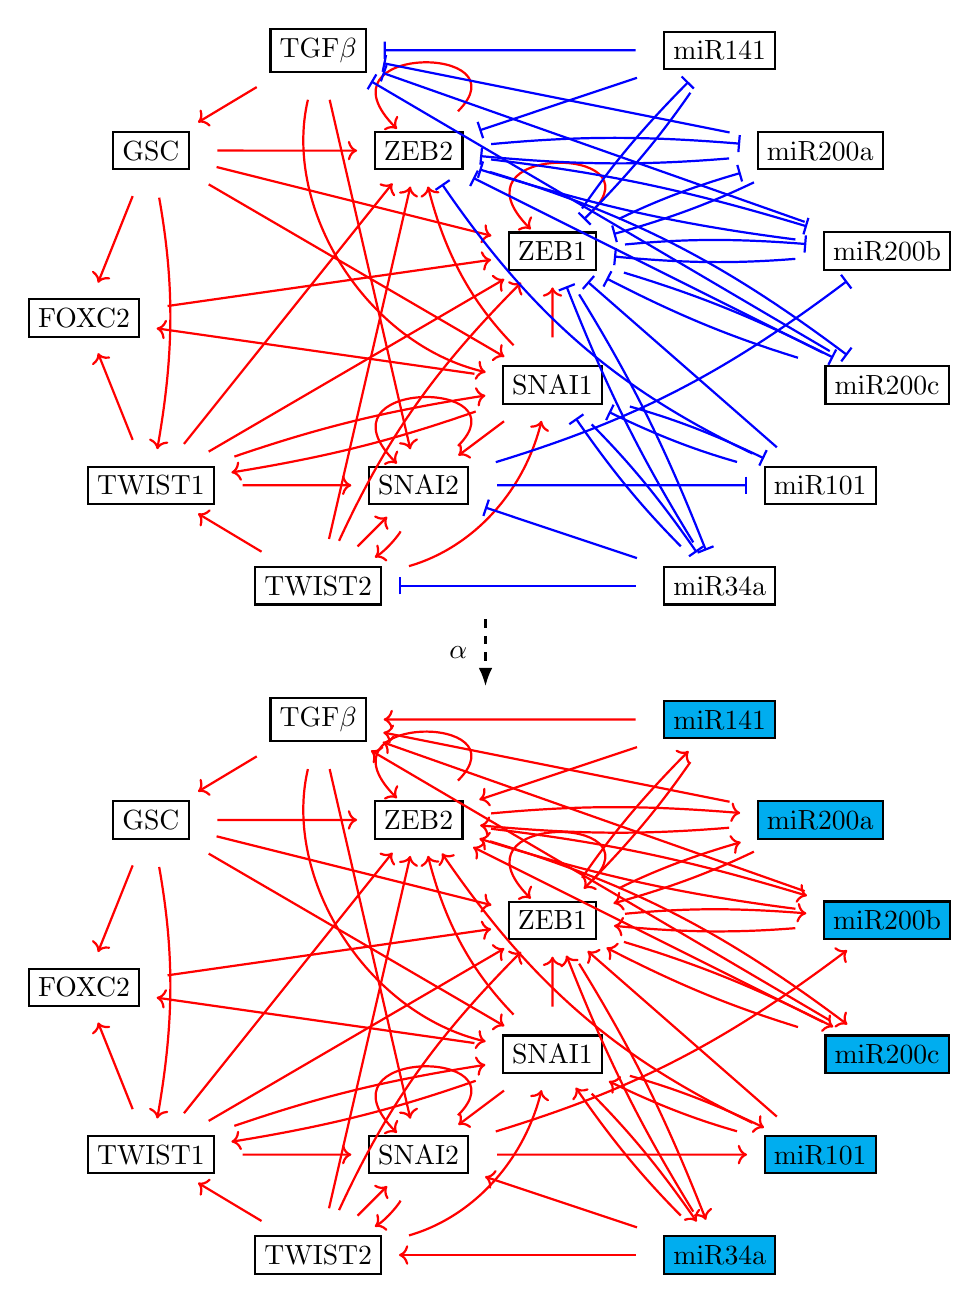
\begin{tikzpicture}[scale=1.7,
    every node/.style={rectangle,fill=white!20,thick,draw},
    blueedge/.style={thick,blue,-|,shorten <=10pt,shorten >=6pt},
    rededge/.style={thick,red,->,shorten <=10pt,shorten >=6pt},
    textbox/.style={draw=none, fill=none, midway}
]
\node (tgf)    at (1.75,4)   {TGF$\beta$};
\node (gsc)    at (0.5,3.25)   {GSC};
\node (foxc2)  at (0,2)     {FOXC2};
\node (tw1)    at (0.5,0.75)   {TWIST1};
\node (tw2)    at (1.75,0) {TWIST2};
\node (zeb2)   at (2.5,3.25) {ZEB2};
\node (zeb1)   at (3.5,2.5)  {ZEB1};
\node (snai1)  at (3.5,1.5)  {SNAI1};
\node (snai2)  at (2.5,0.75)   {SNAI2};
\node (mir141)  at (4.75,4) {miR141};
\node (mir200a) at (5.5,3.25)   {miR200a};
\node (mir200b) at (6,2.5){miR200b};
\node (mir200c) at (6,1.5){miR200c};
\node (mir101)  at (5.5,0.75)    {miR101};
\node (mir34a)   at (4.75,0) {miR34a};

\path[rededge]
    (foxc2) edge (zeb1)
    (snai1) edge (foxc2)
    (snai1) edge (snai2)
    (snai1) edge[bend left=5] (tw1)
    (snai1) edge (zeb1)
    (snai1) edge[bend left=15] (zeb2)
    (snai2) edge[loop] (snai2)
    (snai2) edge[bend left=20] (tw2)
    (tw1) edge (foxc2)
    (tw1) edge[bend left=5] (snai1)
    (tw1) edge (snai2)
    (tw1) edge (zeb1)
    (tw1) edge (zeb2)
    (tw2) edge[bend right] (snai1)
    (tw2) edge (snai2)
    (tw2) edge (tw1)
    (tw2) edge[bend left=10] (zeb1)
    (tw2) edge (zeb2)
    (zeb1) edge[loop] (zeb1)
    (zeb2) edge[loop] (zeb2)
    (gsc) edge (snai1)
    (gsc) edge[bend left=10] (tw1)
    (gsc) edge (foxc2)
    (gsc) edge (zeb1)
    (gsc) edge (zeb2)
    (tgf) edge (gsc)
    (tgf) edge[bend right=45] (snai1)
    (tgf) edge (snai2);

\path[blueedge]
    (mir101) edge (zeb1)
    (mir101) edge[bend left=15] (zeb2)
    (mir101) edge[bend left=5] (snai1)
    (mir141) edge[bend left=5] (zeb1)
    (mir141) edge (zeb2)
    (mir141) edge (tgf)
    (mir200a) edge[bend left=5] (zeb1)
    (mir200a) edge[bend left=5] (zeb2)
    (mir200a) edge (tgf)
    (mir200b) edge[bend left=5] (zeb1)
    (mir200b) edge[bend left=5] (zeb2)
    (mir200b) edge (tgf)
    (mir200c) edge[bend left=5] (zeb1)
    (mir200c) edge (zeb2)
    (mir200c) edge (tgf)
    (mir34a) edge[bend left=5] (snai1)
    (mir34a) edge (snai2)
    (mir34a) edge (tw2)
    (mir34a) edge[bend left=5] (zeb1)
    (snai1) edge[bend left=5] (mir34a)
    (snai1) edge[bend left=5] (mir101)
    (snai2) edge (mir101)
    (snai2) edge[bend right=10] (mir200b)
    (zeb1) edge[bend left=5] (mir141)
    (zeb1) edge[bend left=5] (mir200b)
    (zeb1) edge[bend left=5] (mir200c)
    (zeb1) edge[bend left=5] (mir200a)
    (zeb1) edge[bend left=5] (mir34a)
    (zeb2) edge[bend left=5] (mir200b)
    (zeb2) edge[bend left=10] (mir200c)
    (zeb2) edge[bend left=5] (mir200a);

\begin{scope}[yshift=-5cm]
\node (tgf_2)    at (1.75,4)   {TGF$\beta$};
\node (gsc_2)    at (0.5,3.25)   {GSC};
\node (foxc2_2)  at (0,2)     {FOXC2};
\node (tw1_2)    at (0.5,0.75)   {TWIST1};
\node (tw2_2)    at (1.75,0) {TWIST2};
\node (zeb2_2)   at (2.5,3.25) {ZEB2};
\node (zeb1_2)   at (3.5,2.5)  {ZEB1};
\node (snai1_2)  at (3.5,1.5)  {SNAI1};
\node (snai2_2)  at (2.5,0.75)   {SNAI2};
\node [fill=cyan] (mir141_2)  at (4.75,4) {miR141};
\node [fill=cyan] (mir200a_2) at (5.5,3.25)   {miR200a};
\node [fill=cyan] (mir200b_2) at (6,2.5){miR200b};
\node [fill=cyan] (mir200c_2) at (6,1.5){miR200c};
\node [fill=cyan] (mir101_2)  at (5.5,0.75)    {miR101};
\node [fill=cyan] (mir34a_2)   at (4.75,0) {miR34a};

\path[rededge]
    (foxc2_2) edge (zeb1_2)
    (snai1_2) edge (foxc2_2)
    (snai1_2) edge (snai2_2)
    (snai1_2) edge[bend left=5] (tw1_2)
    (snai1_2) edge (zeb1_2)
    (snai1_2) edge[bend left=15] (zeb2_2)
    (snai2_2) edge[loop] (snai2_2)
    (snai2_2) edge[bend left=20] (tw2_2)
    (tw1_2) edge (foxc2_2)
    (tw1_2) edge[bend left=5] (snai1_2)
    (tw1_2) edge (snai2_2)
    (tw1_2) edge (zeb1_2)
    (tw1_2) edge (zeb2_2)
    (tw2_2) edge[bend right] (snai1_2)
    (tw2_2) edge (snai2_2)
    (tw2_2) edge (tw1_2)
    (tw2_2) edge[bend left=10] (zeb1_2)
    (tw2_2) edge (zeb2_2)
    (zeb1_2) edge[loop] (zeb1_2)
    (zeb2_2) edge[loop] (zeb2_2)
    (gsc_2) edge (snai1_2)
    (gsc_2) edge[bend left=10] (tw1_2)
    (gsc_2) edge (foxc2_2)
    (gsc_2) edge (zeb1_2)
    (gsc_2) edge (zeb2_2)
    (tgf_2) edge (gsc_2)
    (tgf_2) edge[bend right=45] (snai1_2)
    (tgf_2) edge (snai2_2)
    (mir101_2) edge (zeb1_2)
    (mir101_2) edge[bend left=15] (zeb2_2)
    (mir101_2) edge[bend left=5] (snai1_2)
    (mir141_2) edge[bend left=5] (zeb1_2)
    (mir141_2) edge (zeb2_2)
    (mir141_2) edge (tgf_2)
    (mir200a_2) edge[bend left=5] (zeb1_2)
    (mir200a_2) edge[bend left=5] (zeb2_2)
    (mir200a_2) edge (tgf_2)
    (mir200b_2) edge[bend left=5] (zeb1_2)
    (mir200b_2) edge[bend left=5] (zeb2_2)
    (mir200b_2) edge (tgf_2)
    (mir200c_2) edge[bend left=5] (zeb1_2)
    (mir200c_2) edge (zeb2_2)
    (mir200c_2) edge (tgf_2)
    (mir34a_2) edge[bend left=5] (snai1_2)
    (mir34a_2) edge (snai2_2)
    (mir34a_2) edge (tw2_2)
    (mir34a_2) edge[bend left=5] (zeb1_2)
    (snai1_2) edge[bend left=5] (mir34a_2)
    (snai1_2) edge[bend left=5] (mir101_2)
    (snai2_2) edge (mir101_2)
    (snai2_2) edge[bend right=10] (mir200b_2)
    (zeb1_2) edge[bend left=5] (mir141_2)
    (zeb1_2) edge[bend left=5] (mir200b_2)
    (zeb1_2) edge[bend left=5] (mir200c_2)
    (zeb1_2) edge[bend left=5] (mir200a_2)
    (zeb1_2) edge[bend left=5] (mir34a_2)
    (zeb2_2) edge[bend left=5] (mir200b_2)
    (zeb2_2) edge[bend left=10] (mir200c_2)
    (zeb2_2) edge[bend left=5] (mir200a_2);
\end{scope}
\draw[dashed, thick] (3,-0.25) -- (3,-0.75) 
    node[textbox, left=1mm] {$\alpha$};
\end{tikzpicture}
\label{fig:EMT22N}
\end{figure}

\end{document}
